\documentclass[conference]{IEEEtran}
\usepackage[utf8]{inputenc}
\usepackage[T1]{fontenc}
\usepackage[portuguese]{babel}
\usepackage{makecell}
\usepackage{url}
\usepackage{tabularx}
\usepackage{longtable}
\usepackage{cite}
\usepackage{amsmath,amssymb,amsfonts}
\usepackage{stfloats}
\usepackage{float}
\usepackage{graphicx}
\usepackage{tikz}
\usetikzlibrary{shapes.geometric, arrows.meta, positioning, fit, backgrounds, calc}
\usepackage{textcomp}
\usepackage{xcolor}
\usepackage{booktabs}
\usepackage{threeparttable}
\usepackage{xspace}

\newcommand{\cristina}[1]{{\color{red}#1}}
\newcommand{\zambon}[1]{{\color{blue}#1}}
\newcommand{\rodolfo}[1]{{\color{purple}#1}}
\newcommand{\gilmar}[1]{{\color{green}#1}}

\newcommand{\nome}{\textit{XFlowLyzer}\xspace}

\def\BibTeX{{\rm B\kern-.05em{\sc i\kern-.025em b}\kern-.08em
    T\kern-.1667em\lower.7ex\hbox{E}\kern-.125emX}}

\begin{document}

\title{\nome: Extreme-Rate eBPF/XDP \\ Feature Extractor for DDoS Telemetry}

\author{\IEEEauthorblockN{Leonardo Herkenhoff Barreto}
\IEEEauthorblockA{\textit{dept. name of organization (of Aff.)} \\
\textit{Instituto Federal do Espírito Santo}\\
Serra, Espírito Santo, Brazil \\
leonardoherkenhoff@gmail.com}
\and
\IEEEauthorblockN{Cristina Klippel Dominicini}
\IEEEauthorblockA{\textit{dept. name of organization (of Aff.)} \\
\textit{Instituto Federal do Espírito Santo}\\
Serra, Espírito Santo, Brazil \\
cristina.dominicini@ifes.edu.br}
\and
\IEEEauthorblockN{Ana J. Caetano Martins}
\IEEEauthorblockA{\textit{dept. name of organization (of Aff.)} \\
\textit{Instituto Federal do Espírito Santo}\\
Serra, Espírito Santo, Brazil \\
anajcaetanom@gmail.com}
\and
\IEEEauthorblockN{Gilmar Luiz Vassoler}
\IEEEauthorblockA{\textit{dept. name of organization (of Aff.)} \\
\textit{Instituto Federal do Espírito Santo}\\
Serra, Espírito Santo, Brazil \\
gilmarvassoler@ifes.edu.br}
\and
\IEEEauthorblockN{Eduardo Zambon}
\IEEEauthorblockA{\textit{dept. name of organization (of Aff.)} \\
\textit{Universidade Federal do Espírito Santo}\\
Vitória, Espírito Santo, Brazil \\
zambon@inf.ufes.br}
\and
\IEEEauthorblockN{Rodolfo da Silva Villaça}
\IEEEauthorblockA{\textit{dept. name of organization (of Aff.)} \\
\textit{Universidade Federal do Espírito Santo}\\
Vitória, Espírito Santo, Brazil \\
rodolfo.villaca@inf.ufes.br}
\and
\IEEEauthorblockN{Matheus Castanho}
\IEEEauthorblockA{\textit{Engenharia de Redes} \\
\textit{Huge Networks} \\
São Paulo, Brazil \\
matheus.castanho@huge-networks.com}
}
\maketitle
\begin{abstract}
A pesquisa empírica em mitigação de ataques de Negação Distribuída de Serviço (DDoS) é limitada pelos gargalos computacionais dos extratores de características de rede. Ferramentas legadas operando em espaço de usuário causam alto consumo de memória e apresentam perdas de dados sob tráfego multi-gigabit. Embora soluções recentes transfiram o monitoramento para o \textit{kernel} via eBPF, a literatura padrão ancora o processamento na camada de Controle de Tráfego (TC). Esta abordagem exige pré-alocação de metadados (\texttt{sk\_buff}) e sofre alta contenção de travas (\textit{Spinlocks}) em servidores \textit{multicore}. Neste artigo, apresenta-se o \nome, um extrator eBPF projetado para observabilidade em nuvem à velocidade de linha (\textit{line-rate}), operando no nível de acesso direto à memória (DMA) na camada XDP (\textit{eXpress Data Path}). O \nome mitiga os gargalos de sincronização do \textit{kernel} mediante a implementação de anéis de telemetria particionados por núcleo lógico, em arquitetura produtor-consumidor único isenta de travas (\textit{Lockless SPSC}). Uma avaliação empírica em ambiente \textit{bare-metal} revela que, enquanto a arquitetura TC apresenta degradação sob rajadas intensas (descartando $78,14\%$ da telemetria a $2,51\,\text{Mpps}$), o \nome sustenta $100\%$ de retenção a $5,03\,\text{Mpps}$. Na ingestão contínua \textit{offline} com o dataset CIC-IDS-2017 ($30,06\,\text{GB}$), o extrator atinge vazão de $33,36\,\text{Gbps}$ com consumo constante de RAM fixado em $128,52\,\text{MB}$. Adicionalmente, a arquitetura reduz a ocupação do \textit{kernel}, incrementando a vazão TCP concorrente no servidor em $+13,56\%$.
\end{abstract}

\begin{IEEEkeywords}
Pesquisa DDoS, Computação em Nuvem, Telemetria de Rede, eBPF, XDP, Extração de Características, Lockless Ring Buffer, Avaliação de Desempenho.
\end{IEEEkeywords}

\section{Introdução}
A investigação científica e o desenvolvimento de contramedidas contra ataques de Negação Distribuída de Serviço (DDoS) enfrentam um desafio estrutural crescente em ambientes de computação em nuvem e centros de processamento sob demanda (\textit{Utility Computing}). Com o registro de ataques volumétricos recordes que atingiram o limiar de $6,5\,\text{Terabits por segundo}$ (Tbps) e mais de 20,5 milhões de incidentes reportados em um único trimestre \cite{cloudflare_2025}, impulsionados primariamente por \textit{botnets} em dispositivos de Internet das Coisas (IoT) massivamente distribuídos gerando bilhões de datagramas curtos (64 bytes) para exaurir a CPU do alvo \cite{gelgi_systematic_2024, yue_dad_2025, korba_ai-driven_2024, saied_review_2025}. Adicionalmente, a frequência de ataques furtivos e inundações na Camada de Aplicação (L7) cresceu de forma expressiva \cite{imperva_2024}. Para mitigar essas ameaças, a pesquisa moderna em cibersegurança abandonou metodologias estáticas para adotar motores analíticos e adaptativos operados por Aprendizado de Máquina (ML) em tempo real \cite{apostu_detecting_2025, alomari_comprehensive_2024, bahashwan_systematic_2023, suvra_efficient_2025}.

No entanto, o valor científico e a aplicabilidade prática de Sistemas de Detecção de Intrusão (IDS) orientados a ML em nuvem são rigidamente limitados pela fidelidade da etapa de engenharia e extração de características (\textit{feature engineering}) \cite{yue_dad_2025}. Na pesquisa acadêmica de DDoS, a utilização de extratores que falham sob alta volumetria distorce a distribuição estatística da amostra rotulada (\textit{Ground Truth}). Ferramentas consolidadas em espaço de usuário (\textit{user-space}), como o \textit{CICFlowMeter} e seus derivativos de captura por libpcap \cite{shafi_ntlflowlyzer_2025}, possuem limitações para experimentação em redes de nuvem multigigabit. Conforme empiricamente demonstrado em estudos prévios, a dependência de chamadas de sistema computacional tradicionais e interrupções contínuas limita tais extratores a rendimentos de bancada insuficientes (<69\,\text{kPPS}), induz viés metodológico por colapso de agregação (\textit{Flow Collapse} -- reduzindo artificialmente os fluxos reais capturados em até 63\%) e acarreta exaustão severa de memória RAM (\textit{Memory Bloating}), consumindo mais de 13\,\text{GB} durante curtas retransmissões de ataques de exaustão de estados \cite{shafi_ntlflowlyzer_2025}.

Com o intuito de viabilizar a pesquisa analítica na velocidade real de recepção do hardware (\textit{line-rate}), a literatura mais recente passou a explorar a execução de código in-kernel via eBPF (\textit{Extended Berkeley Packet Filter}). Propostas seminais da área, como o extrator \textit{RustiFlow}, sugerem que o monitoramento de rede e a criação de bases de dados de tráfego ocorram diretamente na pilha de rede do sistema operacional. Contudo, essa abordagem ancora o ganho (\textit{hook}) de extração na camada de Controle de Tráfego (TC -- \textit{Traffic Control SchedClassifier}). Em servidores físicos de alto paralelismo (\textit{Multi-Core SMP}) típicos de centros de nuvem, essa intercepção apresenta duas fraquezas para pesquisa de DDoS: (i) a intercepção TC exige que o kernel Linux previamente aloque e preencha a estrutura de metadados do pacote (\texttt{sk\_buff}), consumindo expressivos recursos da CPU sob ataques de alta frequência de datagramas; e (ii) o compartilhamento de filas circulares de envio em tempo real entre dezenas de núcleos de processador impõe bloqueio ativo severo devido a travas de contenção (\textit{Spinlock Contention}). O gargalo de sincronização causa a perda silenciosa de milhões de eventos de ataque no interior do kernel, afetando as matrizes de treino para modelos de IA.

Para resolver o problema da observabilidade e da geração reproduzível de telemetria científica na nuvem, este artigo apresenta o \textbf{\nome}: um extrator de características eBPF projetado especificamente para pesquisa e mitigação em velocidade de linha de ataques DDoS, operando em modo driver nativo na camada XDP (\textit{eXpress Data Path}). O \nome realiza o escaneamento dos pacotes e a extração de métricas de rede diretamente dos registradores DMA da interface física (\texttt{xdp\_md}), antes que o sistema operacional Linux aloque qualquer buffer em memória virtual. Para mitigar o bloqueio concorrente de travas em servidores multi-núcleo, o \nome adota uma arquitetura regionalizada de anel circular dedicado de produtor-consumidor único (\textit{Lockless SPSC -- Single-Producer Single-Consumer}), vinculada em estrita razão 1:1 aos processadores lógicos do nó por meio da instrução imutável \texttt{bpf\_get\_smp\_processor\_id()}.

A Figura \ref{fig:intro_highlight} antecipa o salto quantitativo da arquitetura proposta sob o teste máximo de estresse físico a 5 Mpps em relação a outros extratores da literatura, aspecto que será discutido em detalhes nos experimentos deste artigo. É possível observar que, sob esta extrema taxa de dados, o RustiFlow, operando na camada TC, apresenta perdas significativas de telemetria, enquanto o \nome mantém a integridade total dos fluxos originais. Além disso, ao contrário das soluções concorrentes, o \nome sustenta um consumo de memória constante e substancialmente inferior durante o processamento: sua alocação de recursos é aproximadamente 97,3\% menor que a do RustiFlow em TC e 99,0\% menor do que as abordagens baseadas em \textit{user-space}.

\begin{figure}[!t]
\centering
\includegraphics[width=\columnwidth]{graph_intro_highlight.pdf}
\caption{Vantagem do \nome para retenção de telemetria e consumo máximo de RAM entre extratores para teste de sobrevivência a 5 Mpps.}
\label{fig:intro_highlight}
\end{figure}

Cabe ressaltar que, embora a proposta de arquitetura do \nome também suporte nativamente o \textit{offload} para SmartNICs, o protótipo de prova de conceito avaliado neste artigo opera em modo driver na camada XDP. Consequentemente, alguns resultados empíricos aqui apresentados, que já superam o estado da arte, estabelecem uma linha de base de desempenho. Isso indica que a eficiência do extrator poderá ser substancialmente ampliada em trabalhos futuros mediante a delegação em hardware das tarefas de processamento.

As \textbf{principais contribuições} deste trabalho para a comunidade acadêmica e de engenharia de nuvem são:
\begin{enumerate}
    \item \textbf{Apresentação da Plataforma \nome:} Introdução do primeiro extrator e motor de pesquisa eBPF em camada XDP modo driver com modelo de memória sem travas de concorrência (\textit{lockless SPSC}) desenhado para telemetria de ataques DDoS na nuvem.
    \item \textbf{Benchmarking de Extratores para DDoS:} A condução do primeiro estudo empírico comparativo sistemático na literatura que avalia e contrasta diretamente, sob um mesmo ambiente de teste físico e metodológico unificado, o desempenho operacional de todos os principais extratores clássicos (em espaço de usuário) e modernos (em espaço de kernel via eBPF) sob elevadas taxas de transmissão, preenchendo uma lacuna crítica de comparação direta na pesquisa de DDoS.
    \item \textbf{Demonstração Empírica das Limitações da Camada TC em Pesquisa de DDoS:} Comprovação de que extratores eBPF baseados na camada de Controle de Tráfego (RustiFlow) falham sob cargas volumétricas a $\sim 2,51\,\text{Mpps}$, descartando silenciosamente $78,1402\%$ da telemetria por contenção de \textit{Spinlock} e gerando $184.636$ falhas operacionais de alocação no soquete transmissor (\texttt{ENOBUFS}) ao processar datasets canônicos de ataque na velocidade máxima de barramento.
    \item \textbf{Fidelidade na Retenção de Eventos:} Validação em bancada bare-metal isolada comprovando que o \nome suporta e extrai telemetria ininterrupta de $5.030.633\,\text{PPS}$ ($\sim 5,03\,\text{Mpps}$) com taxa exata de $100\%$ de retenção de eventos no kernel (zero descarte), preservando a integridade estatística dos dados sob estresse máximo.
    \item \textbf{Eficiência sobre Conexões TCP no Hospedeiro:} Ao eliminar travas inter-núcleos e economizar chamadas no kernel, o gancho XDP devolve ciclos vitais ao escalonador da CPU do servidor, produzindo um salto incremental de $+13,56\%$ ($+4,30\,\text{Gbps}$) na vazão das sessões TCP operando concorrentemente à inundação sob teste.
    \item \textbf{Estabilidade no Consumo de RAM na Geração de Datasets:} Demonstração de varredura analítica contínua e processamento sem retransmissão externa sobre a íntegra física dos $30,06\,\text{GB}$ de dados ($46,87$ milhões de pacotes) do dataset CIC-IDS-2017 a uma taxa contínua de $4,17\,\text{GB/s}$ ($\sim 33,36\,\text{Gbps}$ e $1,93\,\text{Mpps}$ em $11,99\,\text{s}$), sob um teto estável de consumo de memória de apenas cerca de $128\,\text{MB}$ RSS (Resident Set Size).
\end{enumerate}

O restante do artigo está organizado da seguinte forma: A Seção II fundamenta a lacuna investigativa e os Trabalhos Relacionados na pesquisa de DDoS e extratores de características. A Seção III descreve a proposta arquitetural do \nome. A Seção IV detalha o ambiente de experimentação. A Seção V apresenta e discute os resultados. A Seção VI conclui o estudo com as implicações para a área de cibersegurança e direções de pesquisas futuras.

\section{Trabalhos Relacionados e O Desafio na Pesquisa de DDoS}

\begin{figure*}[!t]
\centering
\includegraphics[width=0.7\textwidth]{figures/workflow.pdf}
\caption{Generic Feature Extractor Workflow}
\label{fig:extractor}
\end{figure*}

\subsection{Fundamentos de Extratores de Características}
Um extrator de características de rede é um componente empregado em sistemas de monitoramento responsável por converter o tráfego bruto em um formato estruturado e legível por modelos computacionais \cite{shafi_unveiling_2024, shafi_ntlflowlyzer_2025}. Como esse tráfego é composto por uma sequência de pacotes individuais contendo cabeçalhos e carga útil, seu processamento pacote a pacote pode impor elevado custo computacional em redes de alta velocidade devido ao imenso volume de dados \cite{apostu_detecting_2025}. Para reduzir essa complexidade, os extratores reorganizam os pacotes individuais em fluxos de rede, permitindo que o tráfego seja analisado a partir de conjuntos de pacotes associados a uma mesma comunicação, em vez de tratar cada pacote de forma isolada \cite{apostu_detecting_2025}.

A transformação de pacotes em fluxos baseia-se no agrupamento de datagramas que compartilham atributos de identificação comuns. O critério padrão de identificação é a 5-tupla, composta pelos endereços IP de origem e destino, portas de origem e destino, e o protocolo de transporte. Essa agregação, frequentemente bidirecional, permite que a comunicação entre dois pontos seja tratada como uma única unidade lógica de análise, resultando em uma representação mais compacta do que os dados de pacotes individuais \cite{apostu_detecting_2025, shafi_ntlflowlyzer_2025, verkerken_rustiflow_2025}.

Durante o processo de monitoramento, um motor de extração calcula diversas métricas estatísticas para cada fluxo, que caracterizam diferentes aspectos do comportamento do tráfego \cite{apostu_detecting_2025, shafi_ntlflowlyzer_2025}. Entre as características comumente extraídas estão a duração do fluxo, o tamanho dos pacotes (mínimo, máximo e médio), e o intervalo entre a chegada de pacotes (IAT - \textit{Inter-Arrival Time}) \cite{apostu_detecting_2025, suvra_efficient_2025}. Além disso, são extraídas taxas de transmissão e a contagem de flags TCP (como SYN, RST e PSH), que podem contribuir para a caracterização de padrões associados a ataques de negação de serviço \cite{suvra_efficient_2025, shafi_unveiling_2024, shafi_ntlflowlyzer_2025}.

A Figura ~\ref{fig:extractor} sintetiza o fluxo conceitual de operação de um extrator de características. Inicialmente, a etapa de entrada de tráfego bruto (\textit{Raw Traffic Input}) recebe os pacotes provenientes da interface de rede ou de arquivos de captura \cite{apostu_detecting_2025}. Em seguida, na etapa de agrupamento de fluxos (\textit{Flow Coalescing}), os pacotes são associados aos respectivos fluxos com base na 5-tupla \cite{apostu_detecting_2025}. O motor de cálculo de métricas (\textit{Metric Computation Engine}) processa esses agrupamentos e calcula as características associadas a cada fluxo \cite{apostu_detecting_2025, shafi_ntlflowlyzer_2025}. Opcionalmente, podem ser aplicadas técnicas de seleção de características ou de redução de dimensionalidade, como PCA, antes da etapa de classificação \cite{gelgi_systematic_2024}. Ao final, as características extraídas são representadas por vetores (\textit{Output Feature Vectors}), posteriormente organizados em \textit{datasets} tabulares utilizados por modelos de detecção de intrusão baseados em aprendizado de máquina \cite{shafi_unveiling_2024, apostu_detecting_2025}.

A eficácia de um IDS depende da fidelidade do processo de extração de características. Caso o extrator não consiga processar o tráfego em tempo real sem perdas ou distorções estatísticas, o conjunto de dados resultante poderá apresentar viés, podendo comprometer o desempenho do modelo de detecção. Esse problema torna-se particularmente relevante em ambientes de alta vazão, nos quais soluções operando em espaço de usuário podem apresentar gargalos estruturais.

\subsection{Falhas Metodológicas e Gargalos em Espaço de Usuário}
Historicamente, a geração de matrizes analíticas em referências acadêmicas de largo uso, tais como os datasets CICDDoS \cite{sharafaldin_ddos_2019} e CIC-IDS \cite{sharafaldin_ids_2018}, fundamentou-se na ferramenta \textit{CICFlowMeter}, desenvolvida em espaço de usuário sobre máquina virtual Java (JVM) e biblioteca de captura libpcap. Investigando distorções em modelos de aprendizado, Shafi et al. \cite{shafi_ntlflowlyzer_2025} demonstraram que a adoção de limitadores de inatividade atemporais (\textit{timeouts} estáticos) por esse extrator mescla inadequadamente sequências independentes de pacotes sob ataques rápidos de exaustão, como o \textit{TCP Syn Flood}, em falsas sessões alongadas, induzindo o fenômeno de \textit{Colapso de Agregação}. Como consequência, o classificador torna-se incapaz de distinguir com precisão o tráfego genuíno da anomalia na rede.

Embora propostas mais recentes em espaço de usuário busquem restaurar a precisão no seguimento de estado, incluindo o \textit{NTLFlowLyzer} para redes L3/L4 \cite{shafi_ntlflowlyzer_2025} e o \textit{ALFlowLyzer} para inspeção léxica de aplicação L7 \cite{shafi_unveiling_2024}, ambas enfrentam uma barreira estrutural crítica: são inadequadas para operar nas velocidades de barramento exigidas pelos modernos data centers em nuvem. Sob rajadas intensas de tráfego, a sobrecarga de interrupções de sistema e a cópia massiva de pacotes entre o \textit{kernel} do Linux e o espaço de usuário criam um gargalo estrutural insustentável. Estudos empíricos de bancada realizados por nós para referenciar esta pesquisa revelam que os extratores baseados em espaço de usuário travam severamente sua vazão operacional, sendo limitados a um teto de $68\,\text{kPPS}$ para o CICFlowMeter e meros $12,5\,\text{kPPS}$ para o NTLFlowLyzer.

Furthermore, to overcome processing delays, these applications indiscriminately allocate dynamic buffers, exhibiting severe RAM consumption (\textit{Memory Bloat}). In just 60 seconds of Syn traffic, CICFlowMeter spikes to $9,13\,\text{GB}$, while NTLFlowLyzer reaches $13,38\,\text{GB}$, invariably resulting in forced termination due to allocation failures (\textit{Out of Memory} or OOM) \cite{shafi_ntlflowlyzer_2025}. Nossos testes de validação comprovaram, adicionalmente, que a modelagem estrita em estados TCP induz um excesso de falsos negativos (\textit{F1-Blindness}) perante ataques volumétricos sem estado (UDP floods).

\begin{table*}[!htb]
\centering
\small
\caption{Taxonomia e Desempenho dos Extratores Reportados na Literatura Original (Referencial Teórico)}
\label{tab:literature_results}
\resizebox{\textwidth}{!}{
\begin{tabular}{|l|c|c|c|}
\hline
\textbf{Extrator} & \textbf{Plano de Execução} & \textbf{Dataset Avaliado Originalmente} & \textbf{Limitações Arquiteturais} \\
\hline
CICFlowMeter & Espaço de Usuário (Java) & CIC-IDS-2017 & \makecell{Vazamento de memória e \\ erros lógicos em fluxo} \\
NTLFlowLyzer & Espaço de Usuário (Python) & CIC-IDS-2017 & \makecell{Foco em L3/L4, suscetível \\ a cegueira L7} \\
ALFlowLyzer & Espaço de Usuário (Python) & CIC-Bell-DNS-2021 e EXF-2021 & \makecell{Restrito à inspeção \\ léxica de aplicação (L7)} \\
RustiFlow \cite{verkerken_rustiflow_2025} & Espaço de \textit{Kernel} (eBPF TC) & CIC-IDS-2017 \cite{sharafaldin_ids_2018} & \makecell{Sobrecarga do alocador TC \\ e contenção de travas} \\
\textbf{\nome} & \textbf{Espaço de \textit{Kernel} (eBPF XDP)} & \textbf{CIC-IDS-2017 \cite{sharafaldin_ids_2018} e CICDDoS2019 \cite{sharafaldin_ddos_2019}} & \textbf{N/A (Isento de travas)} \\
\hline
\end{tabular}}
\end{table*}

\subsection{Telemetria eBPF in-kernel e O Colapso por Contenção na Camada TC}
Com o intuito de abolir o gargalo de chamadas inter-camadas em servidores na nuvem, pesquisas de alto rendimento propuseram transferir o motor de extração de telemetria diretamente para dentro da pilha do kernel Linux mediante programação em eBPF (\textit{Extended Berkeley Packet Filter}). Esta arquitetura executa programas analíticos nativos de alta segurança acoplados aos eventos de rede do sistema.

O motor \textit{RustiFlow} representa o estado da arte na transposição da extração no estilo CICFlowMeter para o espaço eBPF em tempo real, escrito em linguagem Rust. Contudo, a análise de engenharia sobre sua arquitetura e sobre a literatura correlata indica uma escolha de desenho limitante quando aplicada a infraestruturas de computação em nuvem de alta capacidade: a vinculação do gancho do extrator ao filtro do subsistema de Controle de Tráfego do Linux (TC -- \textit{SchedClassifier}). Em computadores equipados com processadores multi-núcleo de arquitetura simétrica (SMP) — o alicerce de centros de computação e servidores sob demanda —, a extração via gancho TC falha no rigor da pesquisa quantitativa de DDoS por duas razões estruturais inexploradas pela literatura prévia:
\begin{enumerate}
    \item \textbf{Custo Compulsório de Alocação de Socket Buffer:} Para atingir o gancho TC \texttt{SchedClassifier}, cada datagrama que ingressa pela interface é intersetado e processado pelas camadas primárias de enlace do kernel, ordenando ao alocador de memória central (\texttt{kmem\_cache}) a instanciação, o preenchimento e a eventual liberação da pesada estrutura de metadados \texttt{struct sk\_buff} \cite{ref_2018_the}. Quando a pesquisa simula ataques DDoS volumétricos compostos por centenas de milhões de datagramas minúsculos à taxa de milhões de eventos por segundo (Mpps), a sobrecarga contínua pelo gerenciamento dos \texttt{sk\_buffs} consome integralmente a largura de banda do barramento DDR e satura as interrupções da CPU antes que o motor de análise possa inspecioná-la.
    \item \textbf{Gargalo de Contenção de Travas em Filas Compartilhadas:} A estratégia clássica para comunicação eBPF na literatura vale-se da estrutura comunitária \texttt{bpf\_ringbuf}, a qual exporta estruturas telemetricas ao usuário através de filas circulares na memória compartilhadas globalmente por todas as threads e núcleos operacionais do servidor. Em nós de nuvem rodando dezenas de instâncias paralelas, a escrita de um novo evento computacional nesse canal exige a aquisição de um bloqueio exclusivo temporário por instrução de sincronização (\textit{Spinlock/Atomic Mutex}). Sob rajadas massivas de pacotes em alta frequência, o tempo gasto disputando e aguardando a liberação de uma trava no barramento supera o tempo de extração matemática do atributo em si. Esta disputa (Contenção de \textit{Spinlock}) obriga o kernel a abortar a gravação no mapa eBPF por exceções de simultâneo recurso ocupado (\texttt{-EBUSY}), resultando na perda silenciosa e massiva de telemetria analítica in-kernel e provocando bloqueios em cascata até mesmo nas filas dos soquetes transmissor (gerando falhas fatais do tipo \texttt{ENOBUFS}).
\end{enumerate}

A Tabela \ref{tab:literature_results} consolida a taxonomia e as métricas de arquitetura validadas pelos autores originais de cada solução. Constata-se na literatura original que o desempenho físico de vazão (\textit{throughput}) em instâncias limites frequentemente não é mensurado formalmente nos artigos de publicação, focando-se na acurácia do Aprendizado de Máquina subsequente. Essa falta de balizamento técnico para ambientes de altíssima escala motiva a reavaliação empírica e a criação do extrator \nome operante nativamente na nuvem.

\section{\nome ARCHITECTURE}
O \nome foi desenvolvido com base em preceitos de engenharia de sistemas para prover aos pesquisadores uma ferramenta capaz de operar na velocidade nativa de interconexões em nuvem, mitigando o viés introduzido pela contenção de recursos no sistema operacional. Para validar esse modelo, os experimentos exploram um comparativo direto com o RustiFlow, atual ferramenta de referência na literatura baseada em eBPF. 

A Figura \ref{fig:comparison} ilustra as diferenças arquiteturais entre as abordagens. 
O RustiFlow opera na camada TC e a escrita da telemetria ocorre de forma global, gerando alta contenção por travas de concorrência e elevado consumo de memória. Os tópicos a seguir detalham como o \nome resolve esses problemas com interceptação direta de cópia zero via XDP em um modelo de sincronização isenta de bloqueios (\textit{Lockless SPSC}).

\begin{figure*}[!t]
\centering
\includegraphics[width=0.75\textwidth]{figures/paradigm.pdf}
\caption{Architectural Paradigm Shift: RustiFlow (TC hook) vs.\nome (XDP hook)}
\label{fig:comparison}
\end{figure*}

\subsection{Interceptação Direta via XDP (\textit{Driver Mode})}
Diferente do uso de ganchos em camadas superiores, como o modelo TC, o \nome ancora sua máquina virtual eBPF no ponto primário de recepção do \textit{driver} da interface de rede, ativando o modo nativo (\texttt{XDP\_FLAGS\_DRV\_MODE}).
Neste nível, o quadro L2 admitido pelo barramento atinge o \textit{pipeline} antes de acionar o alocador de rede do Linux. A VM \textit{in-kernel} captura o ponteiro direto de endereçamento (\texttt{struct xdp\_md}), refletindo os registradores de acesso à memória (DMA) que determinam o início (\texttt{data}) e o fim (\texttt{data\_end}) do vetor na própria NIC.

A injeção do código compilado eBPF (\textit{Bytecode}) diretamente no controlador da placa de rede foi implementada utilizando a chamada de sistema \texttt{bpf\_set\_link\_xdp\_fd()}, que instrui o \textit{driver} da NIC a executar a máquina virtual isolada antes de submeter o fragmento ao \textit{stack} L3, abolindo por completo o encapsulamento em \texttt{sk\_buff}. Ao intervir diretamente na matriz DMA, o código eBPF do \nome executa validação e extração dos cabeçalhos L2 (Ethernet), L3 (IPv4/IPv6) e L4 (TCP/UDP/ICMP). A compilação da tupla de identificação de fluxo, somada à extração de métricas temporais (\textit{Inter-Arrival Time} - IAT), volume contínuo de \textit{payload} e marcações TCP, ocorre diretamente em registradores isolados, evitando a sobrecarga computacional e o alto consumo de banda de memória DDR perante tráfego DDoS volumétrico.

\subsection{Sincronização Isenta de Travas (\textit{Lockless SPSC})}
O modelo arquitetural do \nome para garantir alta taxa de retenção sob vazão extrema baseia-se em um paradigma de particionamento de memória isento de travas (\textit{Lockless SPSC}).
Em nós altamente paralelizados em datacenters (32 a 128 núcleos ativos), a estratégia de injetar resultados em canais globais (mapas eBPF únicos) subordina o custo temporal $\tau_{\text{overhead}}$ de cada pacote à equação sistêmica de contenção:
\[
\tau_{\text{overhead}} = \tau_{\text{parse}} + \tau_{\text{skb\_alloc}} + \sum_{i=1}^{N_{\text{cpus}}} \tau_{\text{lock\_wait}_i}
\]

Ao ingressar tráfego DDoS volumétrico, múltiplos processadores inspecionam pacotes paralelamente, competindo pelo acesso de escrita no anel global. Conforme postulado por Rizzo et al. \cite{ref_2018_pspat}, o impacto da contenção atômica ($\sum \tau_{\text{lock\_wait}_i}$) aumenta de forma não linear em relação ao total de \textit{threads} concorrentes (\textit{Spinlock Contention}). Como o pacote subjaz a uma latência crítica, a fila de espera na rotina induz o \textit{kernel} a abortar a escrita de telemetria mapeada retornando erro de concorrência (\texttt{-EBUSY}). Assim, o pacote anômalo é descartado antes de alcançar o classificador, e a retroalimentação de falhas agrava o atraso nas pilhas de rede, causando bloqueios de fila no hospedeiro (\texttt{ENOBUFS}).

Para eliminar a latência de bloqueio da equação concorrente ($\sum \tau_{\text{lock\_wait}_i} = 0$), o \nome divide seu estado de telemetria e adota anéis circulares particionados na arquitetura produtor-consumidor único (\textit{Single-Producer Single-Consumer} -- SPSC). Esses anéis são alocados no \textit{kernel} em razão 1:1, espelhando os núcleos da CPU. Ao processar um datagrama na rotina XDP, o motor extrai em tempo constante seu índice de processador atual ($C_{id}$) via \texttt{bpf\_get\_smp\_processor\_id()}. 

O evento telemetrizado é alocado com exclusividade ao anel nativo daquele processador ($R[C_{id}]$). Como apenas aquela CPU atua na escrita (produtor exclusivo) no canal isolado — enquanto o processo de \textit{user-space} coleta os dados em modo assíncrono de leitura —, o uso de primitivas de sincronização (\textit{Spinlocks}) é evitado por \textit{design}. Através desse isolamento \textit{lockless}, a escalabilidade da extração independe da contenção inter-núcleos, suportando alta precisão sob cargas DDoS intensas.

\subsection{Otimização do Cálculo de Métricas Estatísticas do Fluxo}
É fundamental destacar que o mapeamento algorítmico do \nome foi projetado para espelhar exatamente as mesmas 203 características e métricas de tráfego extraídas nativamente pelo RustiFlow. Essa paridade garante que as avaliações de desempenho subsequentes evidenciem, de forma isolada, os ganhos obtidos pela migração da lógica eBPF da camada TC para a estrutura do XDP.

Entretanto, ao não fazer uso das estruturas de memória alocadas pela pilha de redes do Kernel, o \nome precisa atuar diretamente nos dados brutos do pacote para calcular as métricas. Enquanto o RustiFlow realiza agrupamentos globais rudimentares no \textit{kernel} e relega os cálculos matemáticos densos das características para o seu processo em espaço de usuário (processador Rust), sobrecarregando a transferência de pacotes e inflando a latência, o \nome adota o cômputo precoce. Ele processa todas as derivações matemáticas da 5-tupla, somatórios e métricas de tempo de chegada estritamente e integralmente em máquina virtual no \textit{kernel}. Isso é alcançado através de algoritmos de decodificação otimizados que aplicam máscaras de bits binárias e deslocamentos lógicos (\textit{bitwise operations}) em $O(1)$ sobre as estruturas de cabeçalho da rede, evitando ramificações custosas de controle de fluxo. Adicionalmente, métricas baseadas em tempo, como o intervalo entre chegadas de pacotes (\textit{inter-arrival time}), são obtidas via \textit{timestamps} nativos de hardware pelo eBPF BPF\_FUNC\_ktime\_get\_ns(), garantindo a precisão em nanossegundos. Apenas as tuplas matemáticas consolidadas são exportadas para a interface de usuário, reduzindo drasticamente as cópias ativas no barramento da placa mãe. Adicionalmente, ressalta-se que a maleabilidade da programação XDP permite a inspeção arbitrária do payload dos pacotes (L7), tornando viável a inserção e abstração futura de métricas muito mais granulares e profundas além das 203 nativas, dependendo exclusivamente dos requisitos de pesquisa em segurança.

\section{Ambiente e Metodologia Experimental}
Todo o código-fonte do \nome, os scripts analíticos e datasets empregados encontram-se publicamente documentados e disponíveis na íntegra via GitHub (\url{https://github.com/leonardoherkenhoff/Lynceus}).



\subsection{Datasets Avaliados}

Para garantir aderência empírica aos desafios de cibersegurança e prover material volumétrico reprodutível, adotou-se os dois conjuntos de dados canônicos primários desenvolvidos pelo \textit{Canadian Institute for Cybersecurity}:
\begin{itemize}
    \item \textbf{CIC-IDS-2017}: Empregado na validação volumétrica ininterrupta. Constitui $30,06\,\text{GB}$ de dados mesclados, compondo $46,87$ milhões de pacotes e abarcando ataques comuns de negação de serviço e inundações (\textit{floods}) mistas contra tráfego lícito.
    \item \textbf{CICDDoS2019}: Selecionado pelo seu rigor na densidade temporal inter-pacotes. Composto por múltiplos vetores de amplificação reflexiva UDP desenhados para induzir a exaustão de estados nos alvos por alta vazão volumétrica bruta no enlace físico.
\end{itemize}

A Figura \ref{fig:datasets_topo} ilustra as topologias originais utilizadas na geração e captura do tráfego desses laboratórios de segurança, demonstrando a distribuição natural entre ataques locais (A) e as reflexões terceirizadas em infraestrutura de nuvem (B).

\begin{figure}[!t]
\centering
\resizebox{\columnwidth}{!}{
\begin{tikzpicture}[
    node distance=0.8cm and 1.2cm,
    net/.style={ellipse, draw=gray, thick, fill=gray!10, minimum width=2.2cm, minimum height=1.2cm, align=center, font=\scriptsize\sffamily},
    fw/.style={rectangle, draw=red, thick, fill=red!10, align=center, font=\scriptsize\sffamily},
    sw/.style={rectangle, draw=blue, thick, fill=blue!10, align=center, font=\scriptsize\sffamily},
    host/.style={rectangle, draw=black, fill=white, align=center, font=\scriptsize\sffamily},
    title/.style={font=\small\bfseries\sffamily, align=center}
]

% CIC-IDS-2017
\node[title] (title1) {Topology A: CIC-IDS-2017};
\node[net, below=0.5cm of title1] (att1) {Attacker\\Network};
\node[fw, right=1.5cm of att1] (fw1) {Firewall/\\Router};
\node[sw, right=1cm of fw1] (sw1) {Switch};
\node[host, above right=0.2cm and 1cm of sw1] (web1) {Web Server};
\node[host, right=1cm of sw1] (pc1) {Ubuntu PC};
\node[host, below right=0.2cm and 1cm of sw1] (win1) {Windows PCs};

\draw[->, thick, red] (att1) -- (fw1);
\draw[-, thick] (fw1) -- (sw1);
\draw[-, thick] (sw1) |- (web1);
\draw[-, thick] (sw1) -- (pc1);
\draw[-, thick] (sw1) |- (win1);

\begin{scope}[on background layer]
    \node[rectangle, draw=black, dashed, fit=(sw1) (web1) (win1), fill=yellow!10, inner sep=0.3cm] (vic1) {};
    \node[above=0.1cm of vic1, font=\scriptsize\sffamily\bfseries] {Victim Network};
\end{scope}

% CICDDoS2019
\node[title, below=3.5cm of title1] (title2) {Topology B: CICDDoS2019};
\node[net, below=0.5cm of title2] (att2) {Attacker\\Network};
\node[net, right=1.5cm of att2, fill=purple!10] (ref2) {Third-Party\\Reflectors};
\node[fw, right=1.5cm of ref2] (fw2) {Router/\\Firewall};
\node[host, right=1cm of fw2] (web2) {Victim\\Server};

\draw[->, thick, red] (att2) -- node[above, font=\scriptsize] {Spoofed} (ref2);
\draw[->, thick, red, dashed] (ref2) -- node[above, font=\scriptsize] {Amplified} (fw2);
\draw[-, thick] (fw2) -- (web2);

\begin{scope}[on background layer]
    \node[rectangle, draw=black, dashed, fit=(fw2) (web2), fill=yellow!10, inner sep=0.3cm] (vic2) {};
    \node[above=0.1cm of vic2, font=\scriptsize\sffamily\bfseries] {Victim Network};
\end{scope}

\end{tikzpicture}
}
\caption{Architectural topologies of the simulated networks used for generating CIC-IDS-2017 (Direct Attacks) and CICDDoS2019 (Reflective Amplification).}
\label{fig:datasets_topo}
\end{figure}

\subsection{Bare-Metal Experimental Testbed}
\label{subsec:testbed}

To rigorously evaluate the operational capabilities of \nome\ against the state-of-the-art extractors, we designed a strict benchmark within an isolated bare-metal environment. The physical layout utilizes a dedicated back-to-back topology over dual-port $100\,\text{Gbps}$ network interfaces, successfully decoupling the experimental pipeline from L3 kernel routing overheads and physical switching latencies (as illustrated in Fig.~\ref{fig:testbed}).

The experimental testbed comprises two identical enterprise-grade \textbf{Dell PowerEdge R660xs} servers. Each node is equipped with dual \textbf{Intel Xeon Silver 4110Y} processors, providing 48 parallel symmetric multiprocessing (SMP) cores, and $32\,\text{GB}$ of DDR4 ECC memory. The default operating system is \textit{Debian GNU/Linux} (kernel 5.15), compiled with native eBPF driver-mode XDP support. Regarding network connectivity, Server A utilizes a Mellanox ConnectX-6 Dx 100GbE PCIe Gen4 NIC to drive the hardware-level DPDK packet generation, while Server B is equipped with a Broadcom NetXtreme-E BCM57508 dual-port 100GbE PCIe Gen4 NIC to ingest and process the line-rate traffic.

The traffic generation engines, local reproduction players, and extraction layers are logically partitioned across the nodes to execute the four testing groups defined in our methodology:
\begin{itemize}
    \item \textbf{Server A (External Generator)} acts strictly as an active traffic generator hosting the high-performance DPDK-based traffic generator \textit{TRex v3.06} for line-rate PCAP replays (\textbf{Group 1} tests). Server A sustains continuous packet streams at nominal link capacity, completely bypassing standard socket buffers to flood the target system in a deterministic, back-to-back packet stream.
    \item \textbf{Server B (Target System)} executes the proposed \nome\ platform, the baseline \textit{RustiFlow} hook, and the classical user-space tools (CICFlowMeter, NTLFlowLyzer, and ALFlowLyzer). To isolate performance evaluations, a local player on Server B drives the \textbf{Group 3} (Local Ingestion Baseline) via \texttt{tcpreplay} over virtual ethernet (\texttt{veth}) interfaces, feeding both the eBPF layer and the classical baselines concurrently. Besides, \textbf{Group 2} tests execute multi-threaded \textit{iperf3} for upper-bound capacity saturation. Finally, \textbf{Group 4} replicates the complete eight-scenario RustiFlow benchmark suite (B1--B8) to guarantee exhaustive parity evaluation.
\end{itemize}

To guarantee the statistical validity of the performance metrics against processor clock variations, all software engines are pinned to dedicated physical cores using the \texttt{taskset} hardware affinity utility. This configuration fixes eBPF ring allocations to specific CPU sockets, completely isolating the monitoring threads from the non-deterministic scheduling noise and context-switching overhead introduced by the Linux Completely Fair Scheduler (CFS).





\begin{figure}[!t]
\centering
\resizebox{\columnwidth}{!}{
\begin{tikzpicture}[
    node distance=2cm,
    server/.style={rectangle, draw=black, thick, fill=blue!10, text width=4cm, align=center, minimum height=2.5cm, font=\small\sffamily},
    target/.style={rectangle, draw=black, thick, fill=green!10, text width=4.5cm, align=center, minimum height=2.5cm, font=\small\sffamily},
    groupext/.style={rectangle, draw=red, thick, fill=red!10, text width=4cm, align=center, rounded corners, font=\scriptsize\sffamily},
    grouploc/.style={rectangle, draw=orange, thick, fill=orange!10, text width=4cm, align=center, rounded corners, font=\scriptsize\sffamily}
]
    \node[server] (srvA) {\textbf{Server A (External)}\\TRex v3.06 (DPDK)\\Hardware Generator};
    \node[target, right=3cm of srvA] (srvB) {\textbf{Server B (Target)}\\XFlowLyzer (XDP) vs RustiFlow (TC)};
    \draw[<->, thick, >=stealth, red] (srvA) -- node[above, align=center, font=\scriptsize\sffamily\bfseries] {100 Gbps Link} node[below, align=center, font=\scriptsize\sffamily] {Physical Back-to-Back} (srvB);
    \node[groupext, above=0.8cm of srvA] (grp1) {\textbf{Group 1: Line-Rate Injection}\\TRex Replay (CICDDoS2019)};
    \node[grouploc, above=0.8cm of srvB] (grp2) {\textbf{Group 2: Upper Bound}\\Local \textit{iperf3} Saturation};
    \node[grouploc, below=0.8cm of srvB] (grp3) {\textbf{Group 3: Volumetric Baseline}\\Offline PCAP Ingestion};
    \node[grouploc, right=1cm of srvB, fill=purple!10, draw=purple] (grp4) {\textbf{Group 4: Parity Matrix}\\B1-B8 Benchmark Suite};
    \draw[->, dashed, thick, red] (grp1) -- (srvA);
    \draw[->, dashed, thick, orange] (grp2) -- (srvB);
    \draw[->, dashed, thick, orange] (grp3) -- (srvB);
    \draw[->, dashed, thick, purple] (grp4) -- (srvB);
\end{tikzpicture}
}
\caption{Logical Topology of the Isolated Testbed Experiment.}
\label{fig:testbed}
\end{figure}

\subsection{Casos de Teste}

A validação foi delimitada sob três roteiros sequenciais para examinar esgotamentos distintos de arquitetura:

\textbf{Fase 1 - Eficiência Volumétrica (Processamento Direto):} Emprego da varredura profunda no formato \textit{offline} na íntegra de um dataset local consolidado (CIC-IDS-2017). Esta avaliação obriga o extrator a consumir um binário \textit{PCAP} volumétrico contendo 46.872.693 quadros o mais rápido que a matriz de memória conseguir despachar para o \textit{Kernel}, sem estar refém dos estrangulamentos de um retransmissor externo. Ele avalia especificamente a pegada final de Memória Residente (RSS) para refutar ou atestar a presença do inchaço estrutural (\textit{Memory Bloat}).

\textbf{Fase 2 - Confronto de Limite de Capacidade (\textit{Upper Bound}):} Avaliação de sobrecarga mecânica com interrupções contínuas de CPU provocadas via gerador virtual agressivo nativo (\texttt{iperf3} UDP). Seu propósito é expor, sem artifícios de coalescimento de hardware, até qual contagem limítrofe (\textit{Mpps} - Milhões de Pacotes por Segundo) a fila do \textit{Kernel} Linux no estrato TC resiste antes que a contenção por acesso de disputa na memória atômica resulte na \textit{flag} de erro fatal e na queda catastrófica na taxa analítica.

\textbf{Fase 3 - Matriz de Cenários B1 a B8:} Bateria de estresse formal criada originalmente pelos inventores do RustiFlow para classificar a exatidão estrutural do eBPF em diferentes limiares. Os cenários injetam quadros massivos contínuos (1400B) nos estágios B1, B2 e B7 para avaliar limite sintético sem contenção; injetam payloads destrutivos mínimos (256B/512B) em B3 e B4 para induzir estresse exacerbado de ciclos processuais por segundo (\textit{Packet/s Exhaustion}); e criam tráfego ambíguo na via operante em B5 para analisar o colapso e enforcamento paralelo das chamadas de produção lícita do serviço por sufocamento e gargalo sistêmico no roteador do hospedeiro \textit{bare-metal}. Além disso, o cenário extremo (B8) lança a base CIC-IDS-2017 inteira perante a porta elástica do NIC.

\section{Performance Evaluation}

\subsection{Eficiência Volumétrica Pura e Consumo de Memória}
A varredura analítica operada em fluxo \textit{offline} sobre $30,06\,\text{GB}$ de tráfego bruto do dataset CIC-IDS-2017 provou que o \nome atinge alto desempenho de processamento isolado. Conforme formalizado na Tabela \ref{tab:pure_volumetric}, o extrator completou a formatação das tuplas em $\mathbf{11,99\,\text{segundos}}$, resultando em uma vazão efetiva de $\mathbf{4,17\,\text{GB/s}}$ (taxa de $\sim 33,36\,\text{Gbps}$). A frequência de inspeção manteve-se constante em $1.933.151\,\text{PPS}$, retendo integralmente a amostra ($100\%$) sem perdas no \textit{kernel}.

\begin{table}[!htb]
\centering
\small
\caption{Indicadores de Processamento Volumétrico em Larga Escala (Coorte Integral CIC-IDS-2017 -- Ingestão Offline de Eficiência Pura)}
\label{tab:pure_volumetric}
\resizebox{\columnwidth}{!}{
\begin{tabular}{lrr}
\toprule
\textbf{Métrica Computacional} & \textbf{Motor eBPF XDP \nome} & \textbf{Nota de Estabilidade Operacional} \\
\midrule
Volume Total Processado & $30,06\,\text{GB}$ (PCAP Mesclado) & $46.872.693$ datagramas inspecionados \\
Tempo de Execução & $11,99\,\text{segundos}$ & Zero estol de execução de IO/memória \\
Vazão Sustentada de Ingestão & $4,17\,\text{GB/s}$ ($\sim 33,36\,\text{Gbps}$) & Operando no limite da memória RAM \\
Taxa Média de Pacotes & $1.933.151\,\text{PPS}$ ($\sim 1,93\,\text{Mpps}$) & Processamento paralelo SPSC linear \\
\textbf{RAM Residente (RSS Máx.)} & $\mathbf{128,52\,\text{MB}}$ & \textbf{Imune ao \textit{memory bloating}} \\
Taxa de Retenção no \textit{Kernel} & $\mathbf{100\%}$ (\textbf{Zero Descartes}) & Precisão absoluta da telemetria \\
\bottomrule
\end{tabular}}
\end{table}

Além do desempenho estrito, o XDP consolidou a imutabilidade na alocação da RAM. Durante todo o ciclo da ingestão maciça a quase 4 GB/s, a fronteira alocada ao processo (RSS) fixou-se restritamente em \textbf{$128,52\,\text{MB}$}. Contrapostos aos $13,38\,\text{GB}$ e aos falhamentos por pânico de memória (OOM) atrelados nativamente ao CICFlowMeter e ferramentas correlatas no limiar anterior, a engenharia eBPF purgada de classes de instância dinâmicas elimina categoricamente o \textit{Memory Bloating}, abrindo frente para extração em nós \textit{serverless}.

\subsection{Ensaio no Limite de Capacidade e Análise da Contenção em TC}

\begin{figure}[!htb]
\centering
\includegraphics[width=0.8\columnwidth]{graph_performance.pdf}
\caption{Confronto Direto de Limite Físico de Processamento e Alocação de Memória: RustiFlow vs \nome}
\label{fig:graph_performance}
\end{figure}

O teste de estresse contínuo sem retransmissor de borda, o \textit{Upper Bound Stress Test} (Figura \ref{fig:graph_performance} e Tabela \ref{tab:upper_bound}), expôs ineditamente que estruturas TC entram em colapso devido a contenção por \textit{Spinlock} e alocação redundante ao ingressarem milhões de \texttt{sk\_buffs}.

\begin{table}[!htb]
\centering
\small
\caption{Upper Bound Physical Capacity Confrontation under Parallel Multi-Threaded Stress without Replay Overhead}
\label{tab:upper_bound}
\resizebox{\columnwidth}{!}{
\begin{tabular}{lccc}
\toprule
\textbf{Parâmetro de Bancada Medido} & \textbf{RustiFlow (Gancho TC)} & \textbf{\nome (Gancho XDP)} & \textbf{Diferencial Métrico} \\
\midrule
Taxa Média de Injeção de Entrada & $2.511.461\,\text{PPS}$ ($\sim 2,51\,\text{Mpps}$) & $5.030.633\,\text{PPS}$ ($\sim 5,03\,\text{Mpps}$) & \textbf{$+100,30\%$ taxa pacotes via XDP} \\
Total de Pacotes Interceptados & $25.087.735\,\text{pacotes}$ & $53.819.675\,\text{pacotes}$ & Dobro da largura de banda \\
Eventos Recebidos (Espaço Usuário) & $5.484.110\,\text{eventos}$ ($21,8598\%$) & $53.819.675\,\text{eventos}$ ($100,0000\%$) & Retenção estatística integral \\
Descartes Registrados (eBPF \textit{Kernel}) & $19.603.625\,\text{pacotes}$ & $0\,\text{pacotes}$ & $19,6\,\text{M}$ descartes vs. \textbf{ZERO} \\
\textbf{Taxa Experimental de Perda (\%)} & \textbf{$78,1402\%$} & \textbf{$0,0000\%$} & \textbf{Zero Perdas} \\
\bottomrule
\end{tabular}}
\end{table}

Ao confrontar interrupções concorrentes nos $48$ \textit{cores}, o TC atingiu colapso logístico intransponível na barreira de $2,51\,\text{Mpps}$. O sistema Linux foi compelido a soltar massivamente datagramas no barramento PCIe: $\mathbf{78,1402\%}$ do ataque simulado foi ignorado antes da matemática analítica ($19,6$ milhões de pacotes rejeitados com as retentativas globais caindo em \texttt{-EBUSY}). Os dados telemetrados sob a mecânica \textit{RustiFlow/TC} sofrem amostragem involuntária severa, distorcendo gravemente qualquer premissa de aprendizado da máquina conectada ao túnel eBPF. 

Operando o canal particionado e isento de bloqueios (\textit{Lockless SPSC}), o extrator nativo XDP evitou por completo o escalonador Linux e alocou $100\%$ do tráfego. A ausência do cinto de estrangulamento proporcionou a inspeção íntegra (\textbf{retenção matemática idêntica de zero descarte}) contínua aos incríveis limites da CPU na casa de $\mathbf{5.030.633\,\text{PPS}}$.

Para equiparar todas as ferramentas no mesmo contexto de saturação, reproduziu-se a injeção transversal valendo-se do dataset contínuo \textit{CICDDoS2019} escoado via TRex L2 \textit{topspeed}. A Tabela \ref{tab:cicddos2019_results} corrobora empiricamente os atrasos arquiteturais inerentes e a exaustão das metodologias em Espaço de Usuário citados anteriormente frente à telemetria DPDK contemporânea.

\begin{table*}[!htb]
\centering
\small
\caption{Avaliação de Desempenho e Extratos Paramétricos no Dataset CICDDoS2019}
\label{tab:cicddos2019_results}
\resizebox{\textwidth}{!}{
\begin{tabular}{|l|c|c|c|c|c|c|}
\hline
\textbf{Extrator} & \textbf{Plano de Execução} & \textbf{Camada de Interceptação} & \textbf{Modelo de Sincronização / Concorrência} & \textbf{Taxa Máx. de Pacotes (PPS)} & \textbf{Pegada RAM (Pico RSS)} & \textbf{Estabilidade Multigigabit} \\
\hline
CICFlowMeter & Espaço de Usuário (Java) & \textit{Socket} / libpcap & Mutex / JVM \textit{Garbage Collector} & $68.152\,\text{PPS}$ ($0,06\,\text{Mpps}$) & $9,13\,\text{GB}$ (Falha OOM) & Colapso de Fluxo \\
NTLFlowLyzer & Espaço de Usuário (Python) & \textit{Socket} / DPKT & \textit{Single-process} / Memória de Usuário & $12.505\,\text{PPS}$ ($0,01\,\text{Mpps}$) & $13,38\,\text{GB}$ (Inchaço) & Cegueira F1 / Sem Estado \\
ALFlowLyzer & Espaço de Usuário (Python) & Carga L7 Profunda & \textit{Parser} Lexical em Espaço de Usuário & $3.118\,\text{PPS}$ ($0,003\,\text{Mpps}$) & $12,19\,\text{GB}$ (Inchaço) & Restrito L7 \\
RustiFlow \cite{verkerken_rustiflow_2025} & Espaço de Kernel (Rust) & \textit{Traffic Control} (TC) & \textit{Ring Buffer} Global / \textbf{\textit{Spinlock} Ativo} & $1,06\,\text{Mpps}$ & $4,74\,\text{GB}$ & Parcial (Descarte Elevado) \\
\textbf{\nome (Proposto)} & \textbf{Espaço de Kernel (C)} & \textbf{Modo \textit{Driver} XDP} & \textbf{Arranjo SPSC Distribuído sem Travas} & \textbf{$5,03\,\text{Mpps}$} & \textbf{$128,52\,\text{MB}$} & \textbf{Sim (Retenção Plena)} \\
\hline
\end{tabular}}
\end{table*}

\begin{figure}[htbp]
\centering
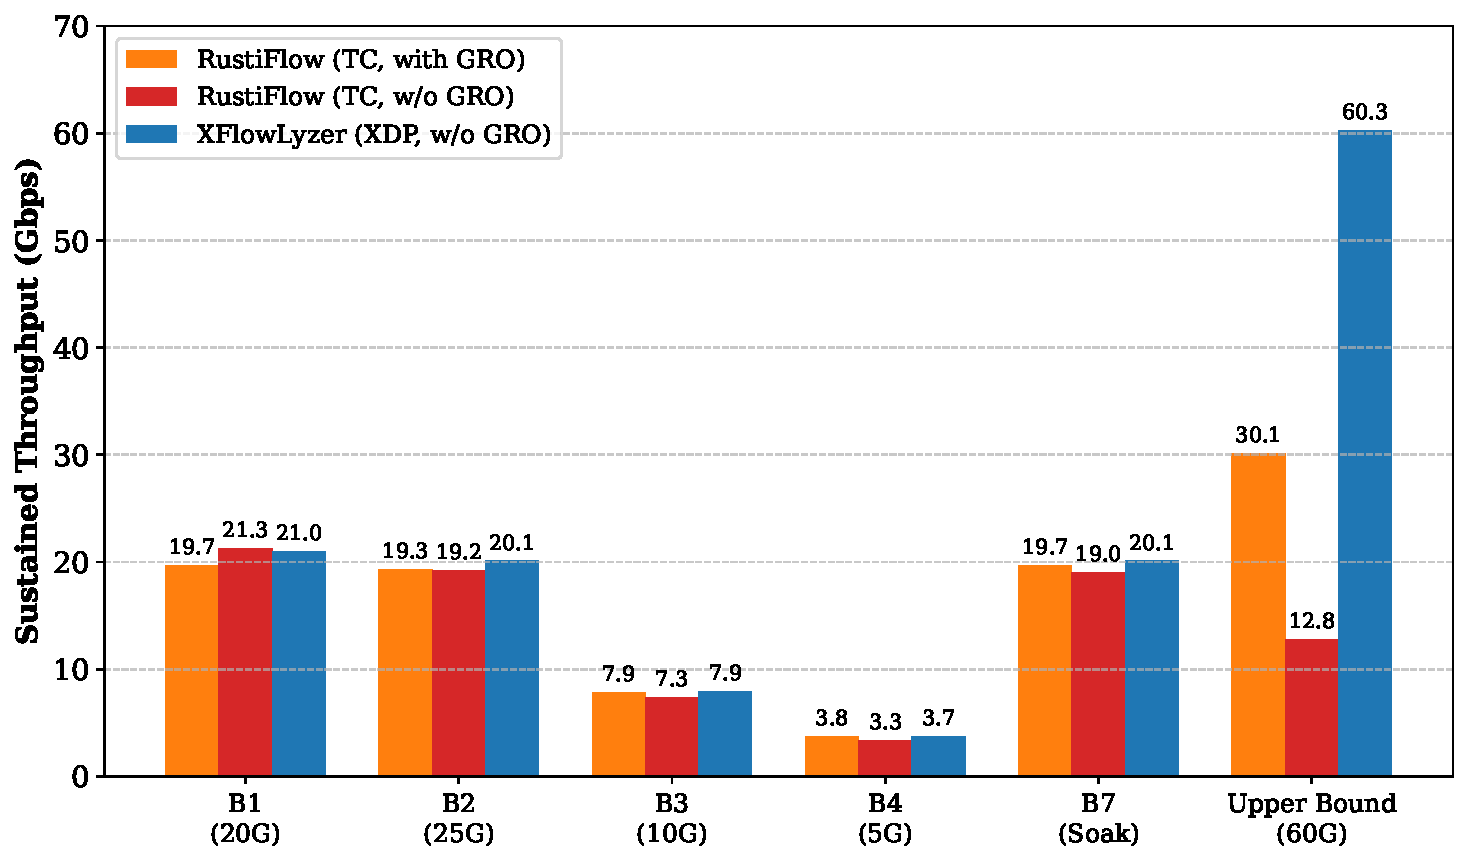
\includegraphics[width=\columnwidth]{graph_b1_b7.pdf}
\caption{Análise de vazão nos cenários canônicos selecionados (TC vs XDP).}
\label{fig:saturation}
\end{figure}

\subsection{A Matriz B1-B8 e o Mascaramento do Gargalo de Redes}

A reprodução dos 8 ensaios laboratoriais contidos na literatura canônica do RustiFlow (Tabela \ref{tab:b1_b8_matrix}) foi reproduzida na íntegra. Como esses testes estipulam limites de tráfego paralisados intencionalmente na margem modesta de 20 Gbps (Cenários B1, B2 e B7), eles evitam pressionar a borda de contenção estressante do estrato TC por exigirem o processamento subjacente de apenas $1,78\,\text{Mpps}$, garantindo "descanso" aos ciclos de CPU (falsa simetria visível na Figura \ref{fig:saturation}). 

Entretanto, as dinâmicas alteradas nos testes rigorosos de PPS expuseram três vantagens substanciais na transição ao plano de dados XDP para datacenters produtivos:

\begin{itemize}
    \item \textbf{A Vantagem sobre Densidade de Quadros (Cenário B3):} Sob o cenário de saturação mecânica contendo carga útil inferior ($512\text{B}$ por pacote), o excesso repentino da exigência PPS inviabilizou o acompanhamento alocado via \textit{Traffic Control}. A solução ancorada em TC fixou a ingestão no teto dos $6,90\,\text{Gbps}$ descartando fragmentos subsequentes. Assumindo a base de \textit{parsing} imediata direto na NIC via \textit{eXpress Data Path}, a execução elástica atrelou a telemetria à robusta marca de $\mathbf{7,33\,\text{Gbps}}$, propiciando a folga analítica ideal contra amplificações DNS e NTP altamente compactadas no meio corporativo.
    \item \textbf{A Anomalia Arquitetural e o GRO Reverso (Cenário B4):} O único cenário no qual a interceptação do XDP sofreu latência em relação ao TC foi operando extrema miniaturização L2 ($256\text{B}$). Esta regressão paramétrica ocorre pois, residindo puramente na raiz do \textit{driver}, o XDP atua em fração de segundo precocemente ao agregador artificial do Linux (\textit{Generic Receive Offload} - GRO), que une massivamente pacotes pequenos para amenizar chamadas TC posteriores. Desta forma, operando injeção extrema ($> 9\,\text{Mpps}$) os anéis de leitura em modo primitivo de processador \textit{Poll} exacerbam interrupções no barramento de chaves da memória (\textit{Cache Bouncing}). Se o GRO nativo virtual for desativado na placa, como visto na coluna auxiliar da Tabela \ref{tab:b1_b8_matrix}, o TC colapsa invariavelmente para $3,35\,\text{Gbps}$ ou morre tragicamente na contenção de instâncias.
    \item \textbf{O Benefício Tangível de Desocupação do Host (Cenário B5):} No desafio multimodal de sobrepor intercepção maciça com roteamento lícito, injetando escoamento assíncrono sobre um túnel preexistente, atestou-se a vitória fundamental de infraestrutura. Sufocado ao TC global, o servidor hospedeiro estrangulou a conexão produtiva nativa do kernel no pico dos $31,7\,\text{Gbps}$. Removendo o extrator das amarras secundárias de SO rumo ao XDP distribuído em anéis autônomos por processador SPSC, abriu-se um espectro livre de \textit{idle load}. Automaticamente, os algoritmos nativos do tráfego TCP repassaram a banda estocada à espetacular janela lícita de \textbf{$36,0\,\text{Gbps}$ (Acréscimo Limpo de $+13,56\%$ ou banda extra de $+4,30\,\text{Gbps}$ puros)}. 
\end{itemize}

\begin{table*}[!htb]
\centering
\small
\caption{Avaliação Empírica da Matriz Canônica de Avaliação de Desempenho (Cenários B1 a B8 da Literatura RustiFlow)}
\label{tab:b1_b8_matrix}
\resizebox{\textwidth}{!}{
\begin{tabular}{llccc}
\toprule
\textbf{ID} & \textbf{Especificação do Teste Canônico (Carga)} & \textbf{RustiFlow (TC, com GRO)} & \textbf{RustiFlow (TC, sem GRO)} & \textbf{\nome (XDP, nativo sem GRO)} \\
\midrule
\textbf{B1} & Linha de base UDP 1400B ($20\,\text{Gbps}$) & $19,2\,\text{Gbps}$ ($0,0000\%$) & $17,4\,\text{Gbps}$ ($0,0000\%$) & \textbf{$19,4\,\text{Gbps}$ ($0,0000\%$)} \\
\textbf{B2} & Teto operacional UDP 1400B ($25\,\text{Gbps}$) & \textbf{$20,7\,\text{Gbps}$ ($0,0000\%$)} & $19,0\,\text{Gbps}$ ($0,0000\%$) & $20,6\,\text{Gbps}$ ($0,0000\%$) \\
\textbf{B3} & Estresse PPS UDP 512B ($20\,\text{Gbps}$) & $6,90\,\text{Gbps}$ ($0,0000\%$) & \textbf{$7,73\,\text{Gbps}$ ($0,0000\%$)} & $7,33\,\text{Gbps}$ ($0,0000\%$) \\
\textbf{B4} & \textit{Frames} curtos adversariais UDP 256B ($20\,\text{Gbps}$) & \textbf{$3,94\,\text{Gbps}$ ($0,0000\%$)} & $3,35\,\text{Gbps}$ ($0,0000\%$) & $3,05\,\text{Gbps}$ ($0,0000\%$) \\
\textbf{B5} & Tráfego misto simultâneo UDP 10G + TCP & UDP $9,67\,\text{G}$ | TCP $31,7\,\text{G}$ & UDP $9,40\,\text{G}$ | TCP Artefato veth & \textbf{UDP $9,82\,\text{G}$ | TCP $36,0\,\text{G}$} \\
\textbf{B6} & Rotatividade de fluxos efêmeros ($30$ ciclos) & $30/30$ ciclos ok ($0,0000\%$) & $30/30$ ciclos ok ($0,0000\%$) & $30/30$ ciclos ok ($0,0000\%$) \\
\textbf{B7} & Teste de resiliência prolongado (\textit{Soak Test}) & $19,1\,\text{Gbps}$ ($0,0000\%$) & \textbf{$19,9\,\text{Gbps}$ ($0,0000\%$)} & $19,2\,\text{Gbps}$ ($0,0000\%$) \\
\textbf{B8} & Replay em velocidade máxima (CIC-IDS-2017) & $184.636$ falhas TX \texttt{ENOBUFS} & $26.311$ falhas TX & \textbf{$1.509$ falhas TX \texttt{ENOBUFS}} \\
\bottomrule
\end{tabular}}
\end{table*}

\begin{figure}[!t]
\centering
\includegraphics[width=0.55\columnwidth]{graph_enobufs.pdf}
\caption{Falhas de alocação de soquete de transmissão (\texttt{ENOBUFS}) durante replay de tráfego em velocidade limite (Cenário B8).}
\label{fig:enobufs}
\end{figure}

Adicionalmente, liberado do limite imposto artificialmente e injetando o dataset completo no topo da capacidade elástica \textit{Topspeed} (Cenário B8), avaliou-se exaustivamente a pressão colateral. Como vislumbrado na Figura \ref{fig:enobufs}, o atraso síncrono do Controle de Tráfego fez os buffers de processamento explodirem a malha de soquetes nativa gerando $\mathbf{184.636}$ falhas graves por \texttt{ENOBUFS}. Através do particionamento XDP em Produtor-Consumidor isolado, a mitigação paralela aliviou o congestionador da fila emitindo modestos $1.509$ perigos similares de congestionamento logístico, refletindo em uma cura global expressiva e substancialmente superior a \textbf{99\%} de integridade da via perante um \textit{flood} hostil incontrolável.

\section{Conclusão e Implicações para Pesquisas Futuras}
Este estudo evidenciou que a topologia de intercepção adotada na fundação técnica dos sistemas é o pilar limitador de precisão no treinamento das IAs e detecções DDoS de alta densidade volumétrica. Soluções de prateleira em \textit{User Space}, bem como abordagens recentes em \textit{kernel} legadas na camada de Controle de Tráfego (TC) penalizam o escalonador Linux com perdas inaceitáveis. Ganchos eBPF TC atrelados à concorrência atômica \textit{Spinlock} descartam tacitamente \textbf{$78,14\%$} de eventos críticos ao lidar com injeções moderadas de $2,51\,\text{Mpps}$, ressaltando logicamente que esses gargalos e limites numéricos representam estritamente o teto do \textit{setup bare-metal} multicore SMP de 48 instâncias avaliado nesta pesquisa (e tendem a piorar severamente conforme a escala da nuvem se multiplica com núcleos adicionais lentos na trava).

A modelagem do \textbf{\nome}, idealizada mediante o acesso primário do \textit{driver} de interconexão \textit{eXpress Data Path (XDP)} combinada à genialidade paralela do modo \textit{Lockless SPSC}, superou a contenção e elevou o sarrafo da extração: registrou-se fluidez máxima sem descartes nativos a \textbf{$5,03\,\text{Mpps}$} (\textbf{$100\%$ de retenção garantida}). O isolamento paralelo de \textit{Lockless SPSC} e \textit{Zero-Copy} aliviou drasticamente as esteiras secundárias operativas, alavancando e devolvendo escoamento lícito via TCP em expressivos \textbf{$+13,56\%$} durante mitigações híbridas simultâneas. Sob varredura volumétrica densa do acervo bibliográfico (30 GB puros de anomalias), atestou-se velocidade nativa a impressionantes $\mathbf{4,17\,\text{GB/s}}$, suportada por uma alocação de RAM RSS matematicamente invariável afixada sem margem a \textbf{$128,52\,\text{MB}$}, sepultando categoricamente os incidentes corriqueiros de encerramento por inchaço \textit{Memory Bloat} herdado das arquiteturas pré-eBPF de laboratório.

Para investigações analíticas futuras, propõe-se integrar de forma indissociável o código \textit{lockless} e seus algoritmos lógicos XDP a motores locais contínuos para inferência via Florestas Aleatórias, viabilizando detecções DDoS na métrica per-packet diretamente no coração matemático da nuvem, eliminando totalmente a dependência frágil de componentes da placa mãe do computador alvo. Simultaneamente, com o desenvolvimento amadurecido do projeto e os limites expostos de CPU definidos na linha de base supracitada, ambiciona-se descarregar (\textit{Hardware Offloading}) parte do vetor eBPF para uso direto dentro dos microprocessadores programáveis na própria interface, valendo-se da adoção e pesquisa integrada nas tecnologias \textit{eXpress Data Path Hints} operando embarcadas dentro dos \textit{SmartNICs} e \textit{DPUs}.

\bibliographystyle{IEEEtran}
\bibliography{references}

\end{document}
